%!TEX root = ../main.tex

\chapter{Invio dei dati al satellite}
\section{Modulazioni utilizzate}
Per inviare i dati al satellite le informazioni sono codificate nelle onde elettromagnetiche attraverso un processo chiamato modulazione.
Tutte le informazioni trasmesse attraverso un mezzo di comunicazione senza fili sono modulate in qualche modo.
Il criterio principale per la scelta dello schema di modulazione è basato sulla massimizzazione del data rate e minimizzazione della potenza trasmessa, della larghezza di banda del canale, dell'errore sul simbolo e resistenza alle interferenze.

Le tecniche di modulazione e demodulazione digitale richiedono una maggiore complessità e un elevato livello di integrazione per trasferire grandi quantità di dati e informazioni.
Un filtraggio eccessivo per migliorare l'efficienza spettrale può ridurre le interferenze ma aumentare il \ac{BER} (Bit Error Rate) a causa della sfocatura dei simboli trasmessi.

Per inviare dati digitali usando una tecnologia analogica, l'emittente genera un sengale portante a una certa frequenza.
Per codificare il segnale digitale nella sinusoide sono poi utilizzate le seguenti tecniche:
\begin{itemize}
  \item Amplitude-shift modulation (keying): varia l'ampiezza (cioè la tensione) del segnale.
  \item Frequency-shift modulation: due (o più) frequenze vicine alla frequenza portante sono utilizzate.
  \item Phase-shift modulation: sposta sistematicamente l'onda portante a intervalli uniformemente spaziati.
\end{itemize}

Oltre alla modulazione i dati vengono trasmessi efficientemente anche utilizzando tecniche di multiplexing.
Il multiplexing consente di combinare più sengali in un singolo canale di trasmissione, massimizzando l'uso della banda e migliorando l'efficienza del sistema.
Esistono due principali approcci al multiplexing: FDM (Frequency Division Multiplexing) e TDM (Time Division Multiplexing).
L'FDM suddivide lo spettro di frequenza in sottocanali, dando a ciascun utente l'utilizzo esclusivo di un sottocanale.
Un problema con FDM è che a un utente è data tutta la frequenza, e se non ha dati da inviare la banda è sprecata, dato che non può essere utilizzata da un altro utente.
Il TDM invece utilizza il time slicing per dare a ciascun utente l'intera banda, ma solo per una frazione di secondo alla volta.
Di nuovo, se l'utente non ha dati da inviare durante il suo timeslice, la banda non è utilizzata, e quindi è sprecata.

La capacità di un satellite Starlink sarà di 20 Gbit/s quando opererà in due polarizzazioni con modulazione 64-\ac{QAM}.
Ad oggi la rete può usare solo una polarizzazione.
Per lavorare con la 64-\ac{QAM} è necessario avere un \ac{SNR} di più di 17dB.
Al momento questo parametro al terminale UT-1 è tra gli 11 e i 12.5 dB, che corrisponde a una 16-32\ac{APSK} e ha un'efficienza spettrale di 4.5 bit/s/Hz al massimo.
Le possibili efficienze spettrali per Starlink sono:

\begin{table}[h]
\centering
\begin{tabular}{|c|c|c|c|}
\hline
\textbf{Modulation} & \textbf{Code rate} & \makecell{\textbf{Spectral efficiency}\\ \textbf{bit/s/Hz}} \\ \hline
QPSK     & 0.5   & 0.989  \\ \hline
8PSK     & 0.75  & 2.228  \\ \hline
8PSK     & 0.833 & 2.479  \\ \hline
16APSK   & 0.666 & 2.637  \\ \hline
16APSK   & 0.75  & 2.967  \\ \hline
32APSK   & 0.9   & 4.453  \\ \hline
64QAM    & 0.772 & 4.5234 \\ \hline
64QAM    & 0.873 & 5.1152 \\ \hline
64QAM    & 0.948 & 5.5547 \\ \hline
\end{tabular}
\caption{Efficienza spettrale di Starlink \cite{rozenvasser_estimation_2023}}
\end{table}

\paragraph{Link budget}
La potenza ricevuta al terminale utente è data da:
\begin{equation}
P_{rx} = P_{tx} + G_{tx} + G_{rx} - L_{tx} - L_{rx} - L_{atm} - L_{p}
\label{eq:received-power}
\end{equation}

In questa equazione, $P_{tx}$ è la potenza del trasmettitore, $G_{tx}$ e $G_{rx}$ sono i guadagni del trasmettitore e del ricevitore, $L_{tx}$ e $L_{rx}$ sono le perdite ai trasmettitori e ricevitori, $L_{atm}$ è la perdita atmosferica, e $L_{p}$ è il path loss introdotto dalla separazione tra il trasmettitore e il ricevitore.

% ROBA SENZA UN CAZZO DI SENSO

% $P_{tx}$ è la potenza del trasmettitore ed è dipendente dall'allocazione dinamica delle risorse $\eta_{a}$ e massa del satellite $m$.

% Il guadagno del trasmettitore $G_{tx}$ è dipendente dalla tecnologia dell'antenna (il diametro $d$ e la lunghezza d'onda $\lambda$):
% \begin{itemize}
%   \item Parabolica: $G_{tx} = 20 \log_{10} (\frac{\eta_{a} \pi d}{\lambda})$
%   \item Phased Array: $G_{tx} = 20 \log_{10} (\frac{4 \eta_{a} \pi \sqrt[3]{m^2}}{\lambda})$
% \end{itemize}

% Il guadagno del ricevitore sul rumore $G_{rx}$ basato sul tipo del terminale utente:
% \begin{itemize}
%   \item Parabolica: $G_{rx} = 5.24 dB$
%   \item Phased Array: $G_{rx} = 10.8 dB$
% \end{itemize}

La perdita atmosferica $L_{atm}$ è dipendente dalla banda di frequenza e pressione atmosferica $P_{atm}$.
Per la Ku/Ka-band $L_{atm} = 0.97 dB/km$ in media.

\begin{figure}[htbp]
  \centering
  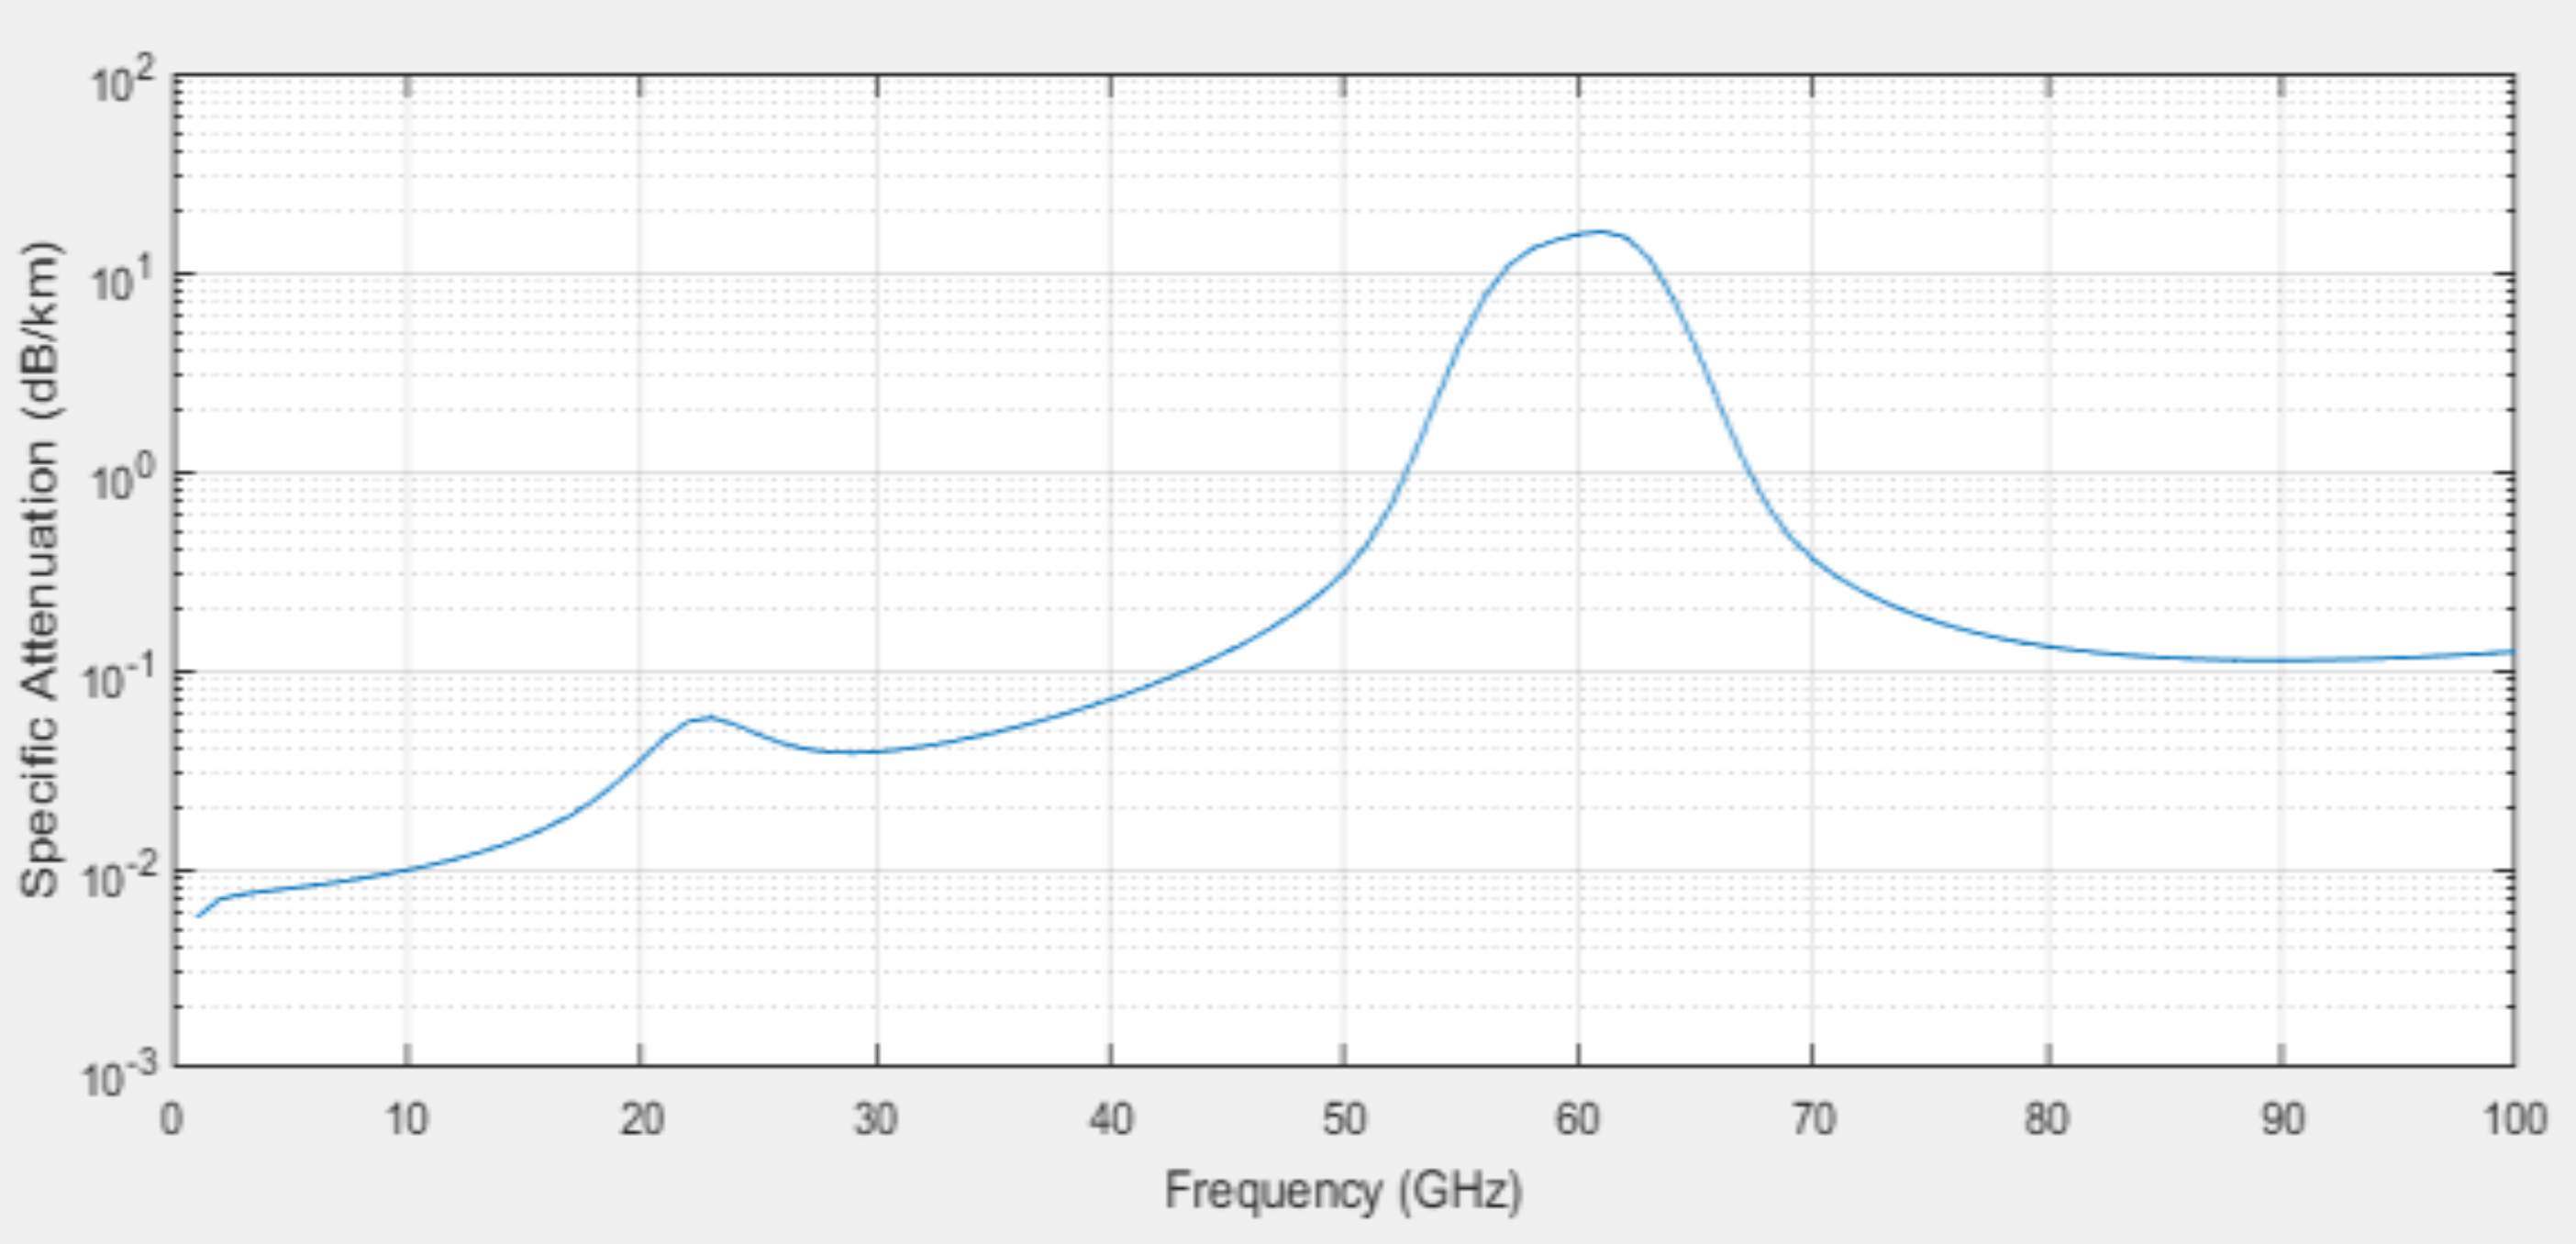
\includegraphics[width=0.8\linewidth]{./res/img/atmospheric_losses_simulation.png}
  \caption{Simulazione delle perdite atmosferiche}
  \label{fig:atmospheric-losses-simulation}
\end{figure}

Osserviamo in figura \ref{fig:atmospheric-losses-simulation} un picco del parametro $L_{atm}$ a 60 GHz.
Per ridurre l'influenza delle perdite atmosferiche è preferibile usare i range di frequenza fino a 53 GHz, che corrisponde al piano di frequenze proposto da SpaceX (tabella \ref{tab:starlink-frequency-allocation-modulation-type}).
Per la trasmissione in uplink si usano le frequenze 14-52.4 GHz e per la trasmissione in downlink le frequenze 10.7-42.5 GHz.
Nella tabella \ref{tab:starlink-frequency-allocation-modulation-type} possiamo anche vedere i tipi di modulazione.
Il tipo di modulazione può cambiare da \ac{BPSK} a 64-\ac{QAM}.

Esiste un trade-off tra la semplicità al ricevitore di un segnale facilmente demodulabile e l'efficienza di quel segnale.
Due delle efficienze di maggior interesse nei sistemi di comunicazione satellitari sono l'efficienza spettrale e l'efficienza energetica.

\paragraph{Efficienza spettrale}
L'efficienza spettrale si riferisce al rapporto tra la velocità dei dati e la larghezza di banda del segnale, che misura quanti bit al secondo possono essere trasmessi per Hertz di larghezza di banda (bps/Hz).
Secondo il teorema della larghezza di banda minima di Nyquist, è possibile trasmettere fino a 2 bps/Hz in banda base senza codifica.
I sistemi ibridi fase-ampiezza a più livelli o sistemi M-ari possono raggiungere efficienze spettrali ancora più elevate a costo di una magagiore complessità. Tuttavia, bisogna comunque tenere presente che la velocità massima dei dati senza errori di questi sistemi è in ultima analisi limitata dal rapporto segnale/rumore (\ac{SNR}), come descritto dal teorema della capacità del canale di Shannon \cite{don_k_lefevre_power-efficient_1989}.

\paragraph{Efficienza energetica}
L'efficienza energetica è il rapporto tra la velocità dei dati e la potenza necessaria per trasmettere i dati senza errori.
Nei sistemi reali, la potenza richiesta dipende anche da fattori quali le figure di rumore, i guadagni dell'antenna e la distanza tra trasmettitore e ricevitore.
Per effettuare confronti relativi, un metodo semplice consiste nel confrontare l'\ac{SNR} richiesto per ottenere lo stesso tasso di errore di bit (\ac{BER}).
Questo approccio consente di confrontare sistemi che sono identici in termini di figura di rumore, perdita di percorso e altri fattori ma differiscono nella modulazione.
La differenza nell'SNR richiesto rivela le prestazioni relative di ciascun tipo di modulazione \cite{don_k_lefevre_power-efficient_1989}.

\begin{table}[h]
\centering
\begin{tabular}{|c|c|c|}
\hline
\textbf{Caratteristica} & \textbf{Uplink} & \textbf{Downlink} \\ \hline
Frequenza (GHz)  & \makecell{14.0-14.5 \\ 27.5-29.1 \\ 29.5-30.0 \\ 47.2-52.4}  & \makecell{10.7-12.7\\17.8-18.6\\18.8-19.3\\37.5-42.5} \\ \hline
Tipo di modulazione  & \makecell{\acs{BPSK},\\M\acs{QAM}} & \makecell{\acs{OQPSK},\\ M\acs{QAM}} \\ \hline
\end{tabular}
\caption{Path loss nello spazio aperto in dB ($L_p$) \cite{rozenvasser_estimation_2023}.}
\label{tab:starlink-frequency-allocation-modulation-type}
\end{table}

% $L_p = 20 \log_{10} (\frac{4 \pi d}{\lambda})$

\begin{figure}[htbp]
  \centering
  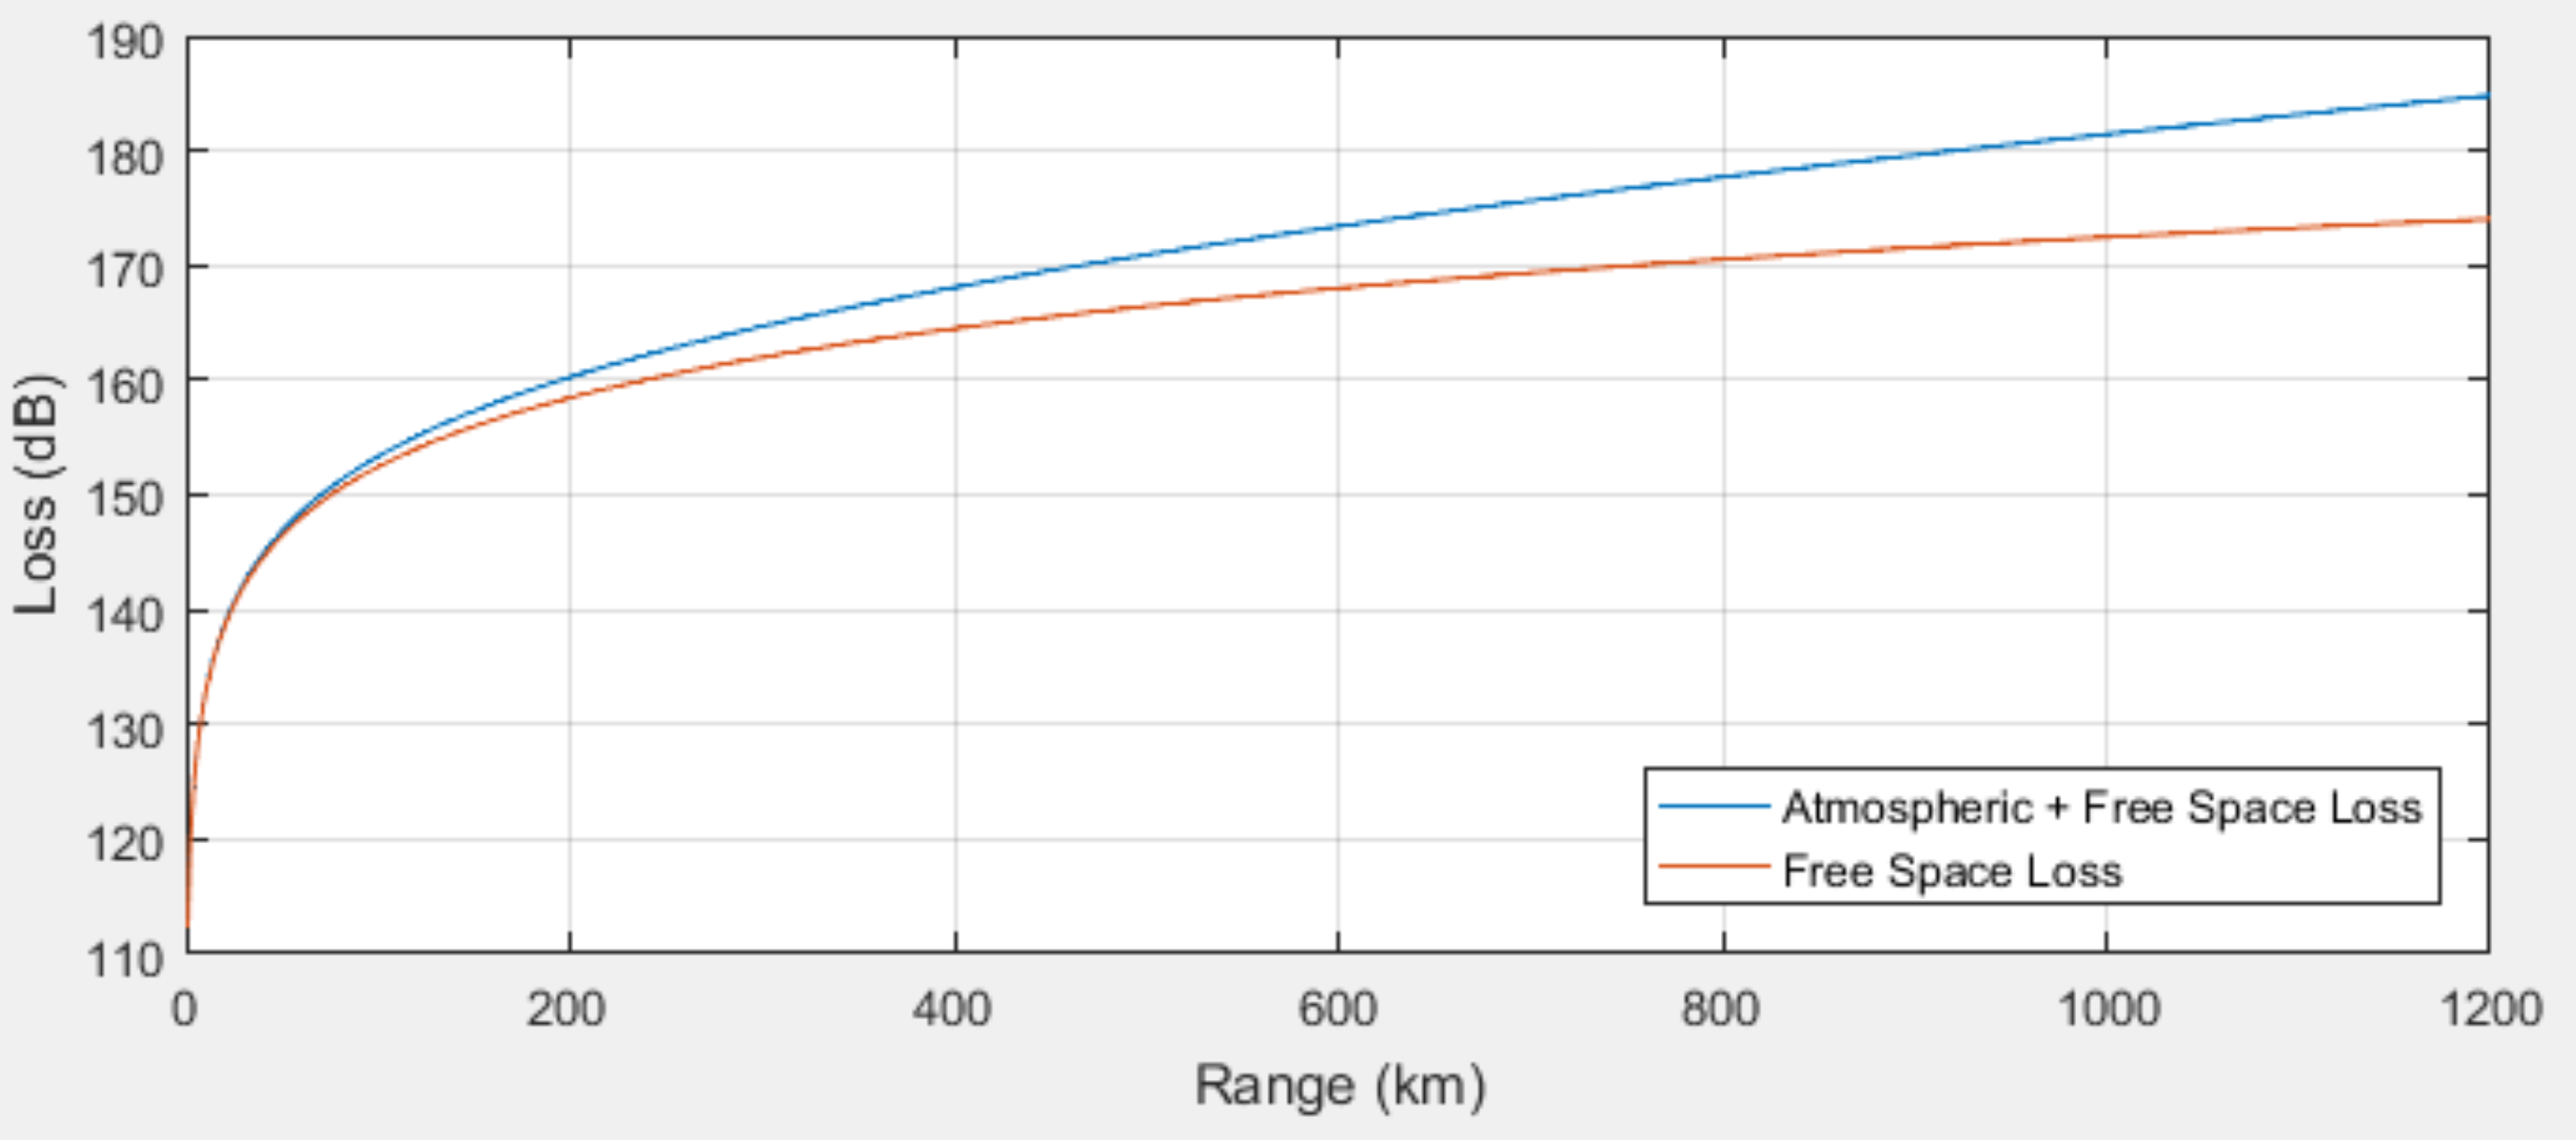
\includegraphics[width=0.8\linewidth]{./res/img/free_space_path_loss_atm_loss.png}
  \caption{Path loss nello spazio libero e perdita atmosferica}
  \label{fig:free-space-path-loss-atm-loss}
\end{figure}

Il path loss nello spazio libero è il contributore principale alla perdita di potenza come si vede in figura \ref{fig:free-space-path-loss-atm-loss}.
Alle altitudini calcolate per i satelliti Starlink, questo valore è di 160-175 dB.
La perdita totale dal path loss nello spazio libero e le perdite atmosferiche sono 165-185 dB.

I risultati della modellazione e del calcolo della dipendenza della potenza ricevuta dal terminale utente dall'altezza dell'orbita del satellite per varie frequenze (da 10 a 50 GHz) sono illustrati nella figura \ref{fig:link-budget-wo-ecc}.

\begin{figure}[htbp]
  \centering
  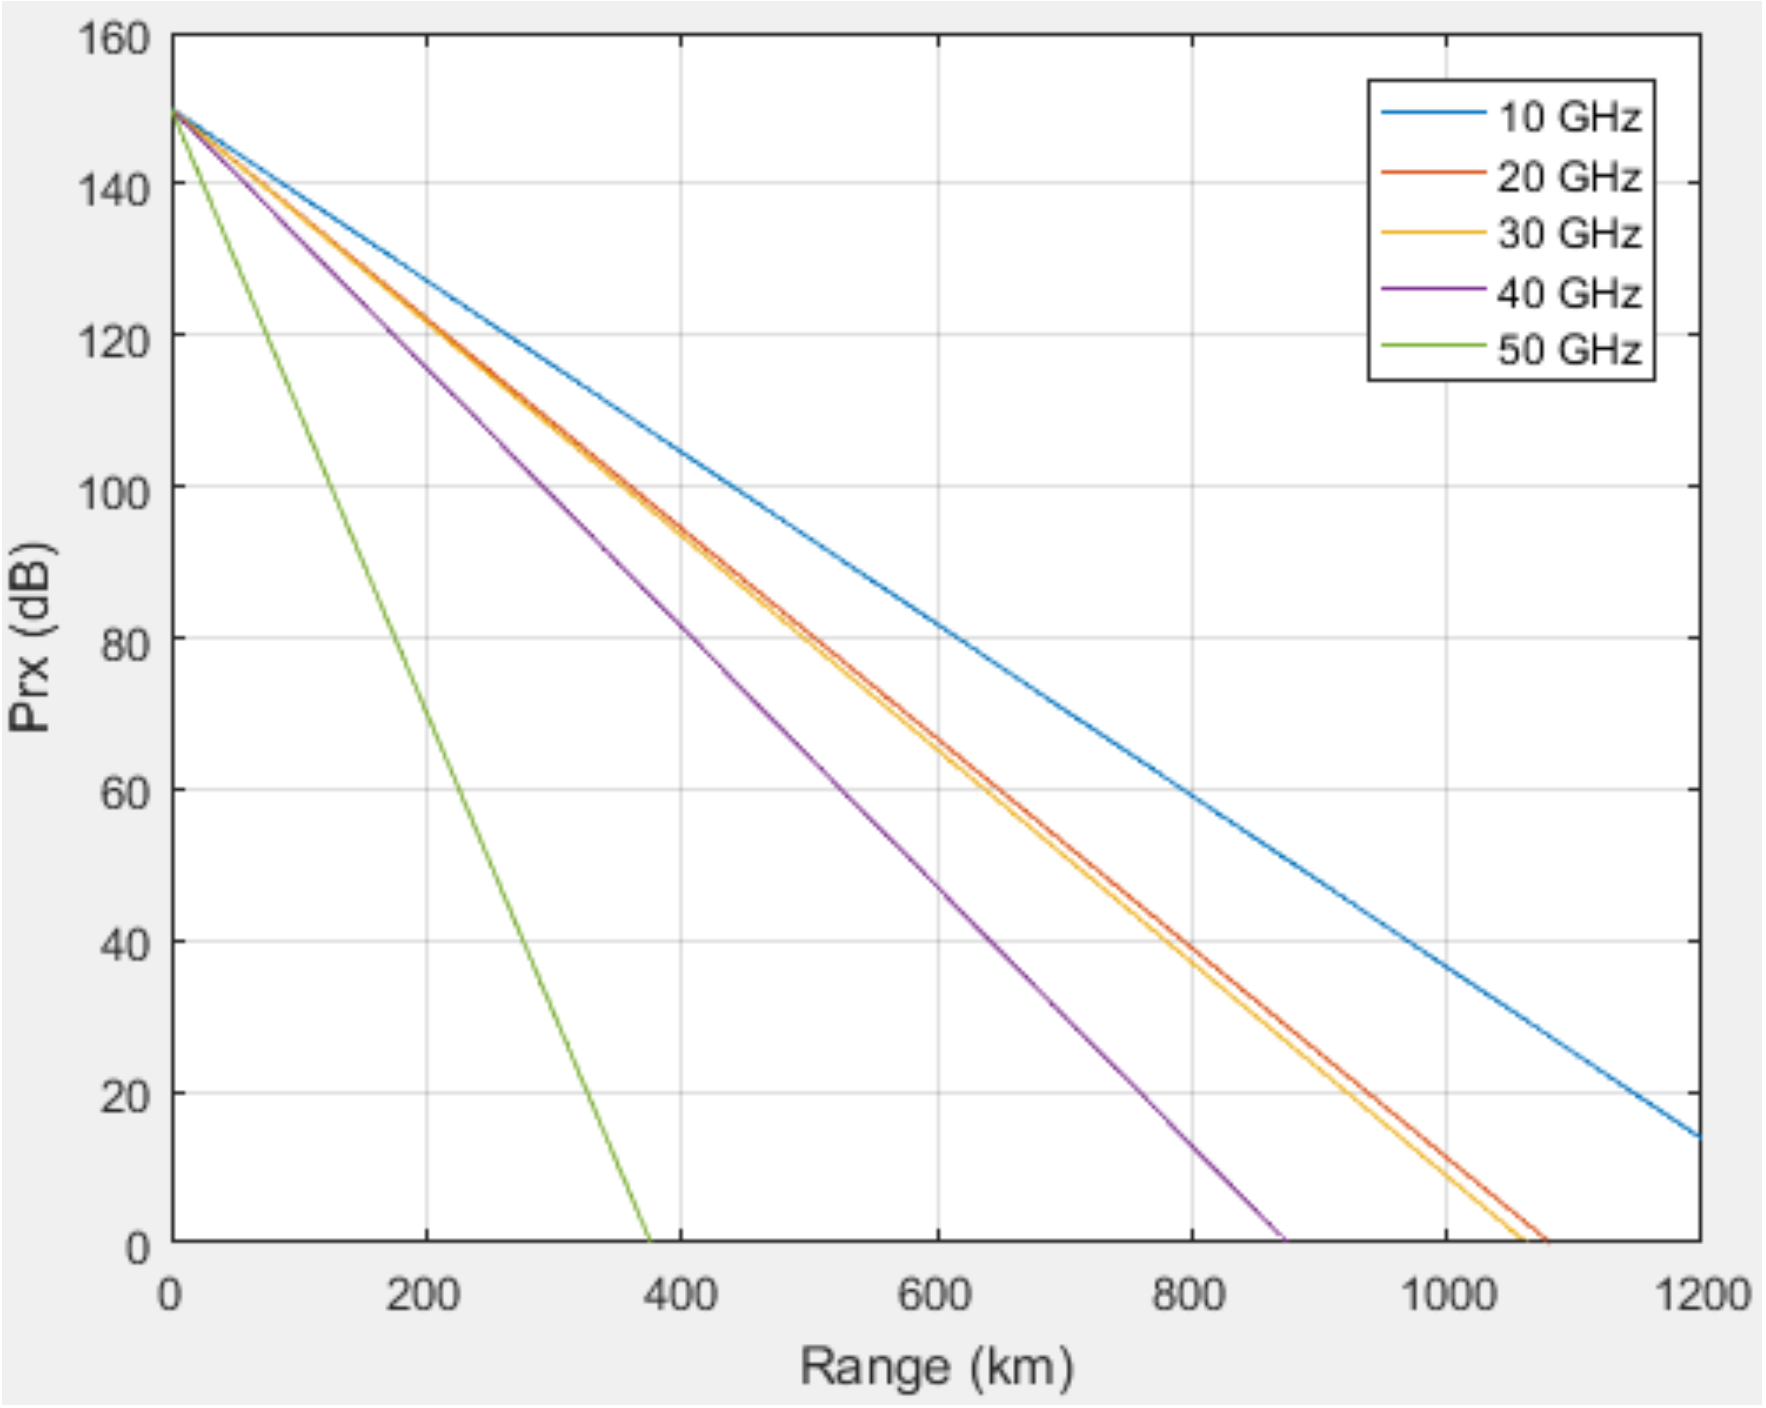
\includegraphics[width=0.8\linewidth]{./res/img/link_budget_wo_ecc.png}
  \caption{Link budget senza \ac{ECC}}
  \label{fig:link-budget-wo-ecc}
\end{figure}

Dalla figura \ref{fig:link-budget-wo-ecc} si può vedere che il valore più alto della potenza del segnale è 150 dB.
Finchè il segnale passa attraverso l'atmosfera gradualmente viene attenuato.
L'attenuazione avviene anche sui dispositivi ricevitori e trasmettitori.
Il grado di attenuazione dipende da molti parametri e limita l'altezza dell'orbita del satellite.

È consuetudine utilizzare un codice a correzione di errore per aumentare l'immunità al rumore dei sistemi.
In questo caso, utilizziamo un codice a correzione di errore per aumentare il link budget.

Aggiungiamo CG, guadagno di codifica dovuto al codice a correzione d'errore (\ac{ECC}), all'equazione (\ref{eq:received-power}) che diventa quindi:

\begin{equation}
  P_{rx} = P_{tx} + G_{tx} + G_{rx} - L_{tx} - L_{rx} - L_{atm} - L_{p} + CG
\end{equation}

I risultati della modellazione e calcolo della dipendenza della potenza ricevuta al terminale utente all'altezza dell'orbita del satellite per frequenze diverse (dai 10 ai 50 GHz), considerando l'uso di un codice di correzione di errore con un guadagno di codice di 10 dB sono mostrate in figura \ref{fig:link-budget-w-ecc}.

\begin{figure}[htbp]
  \centering
  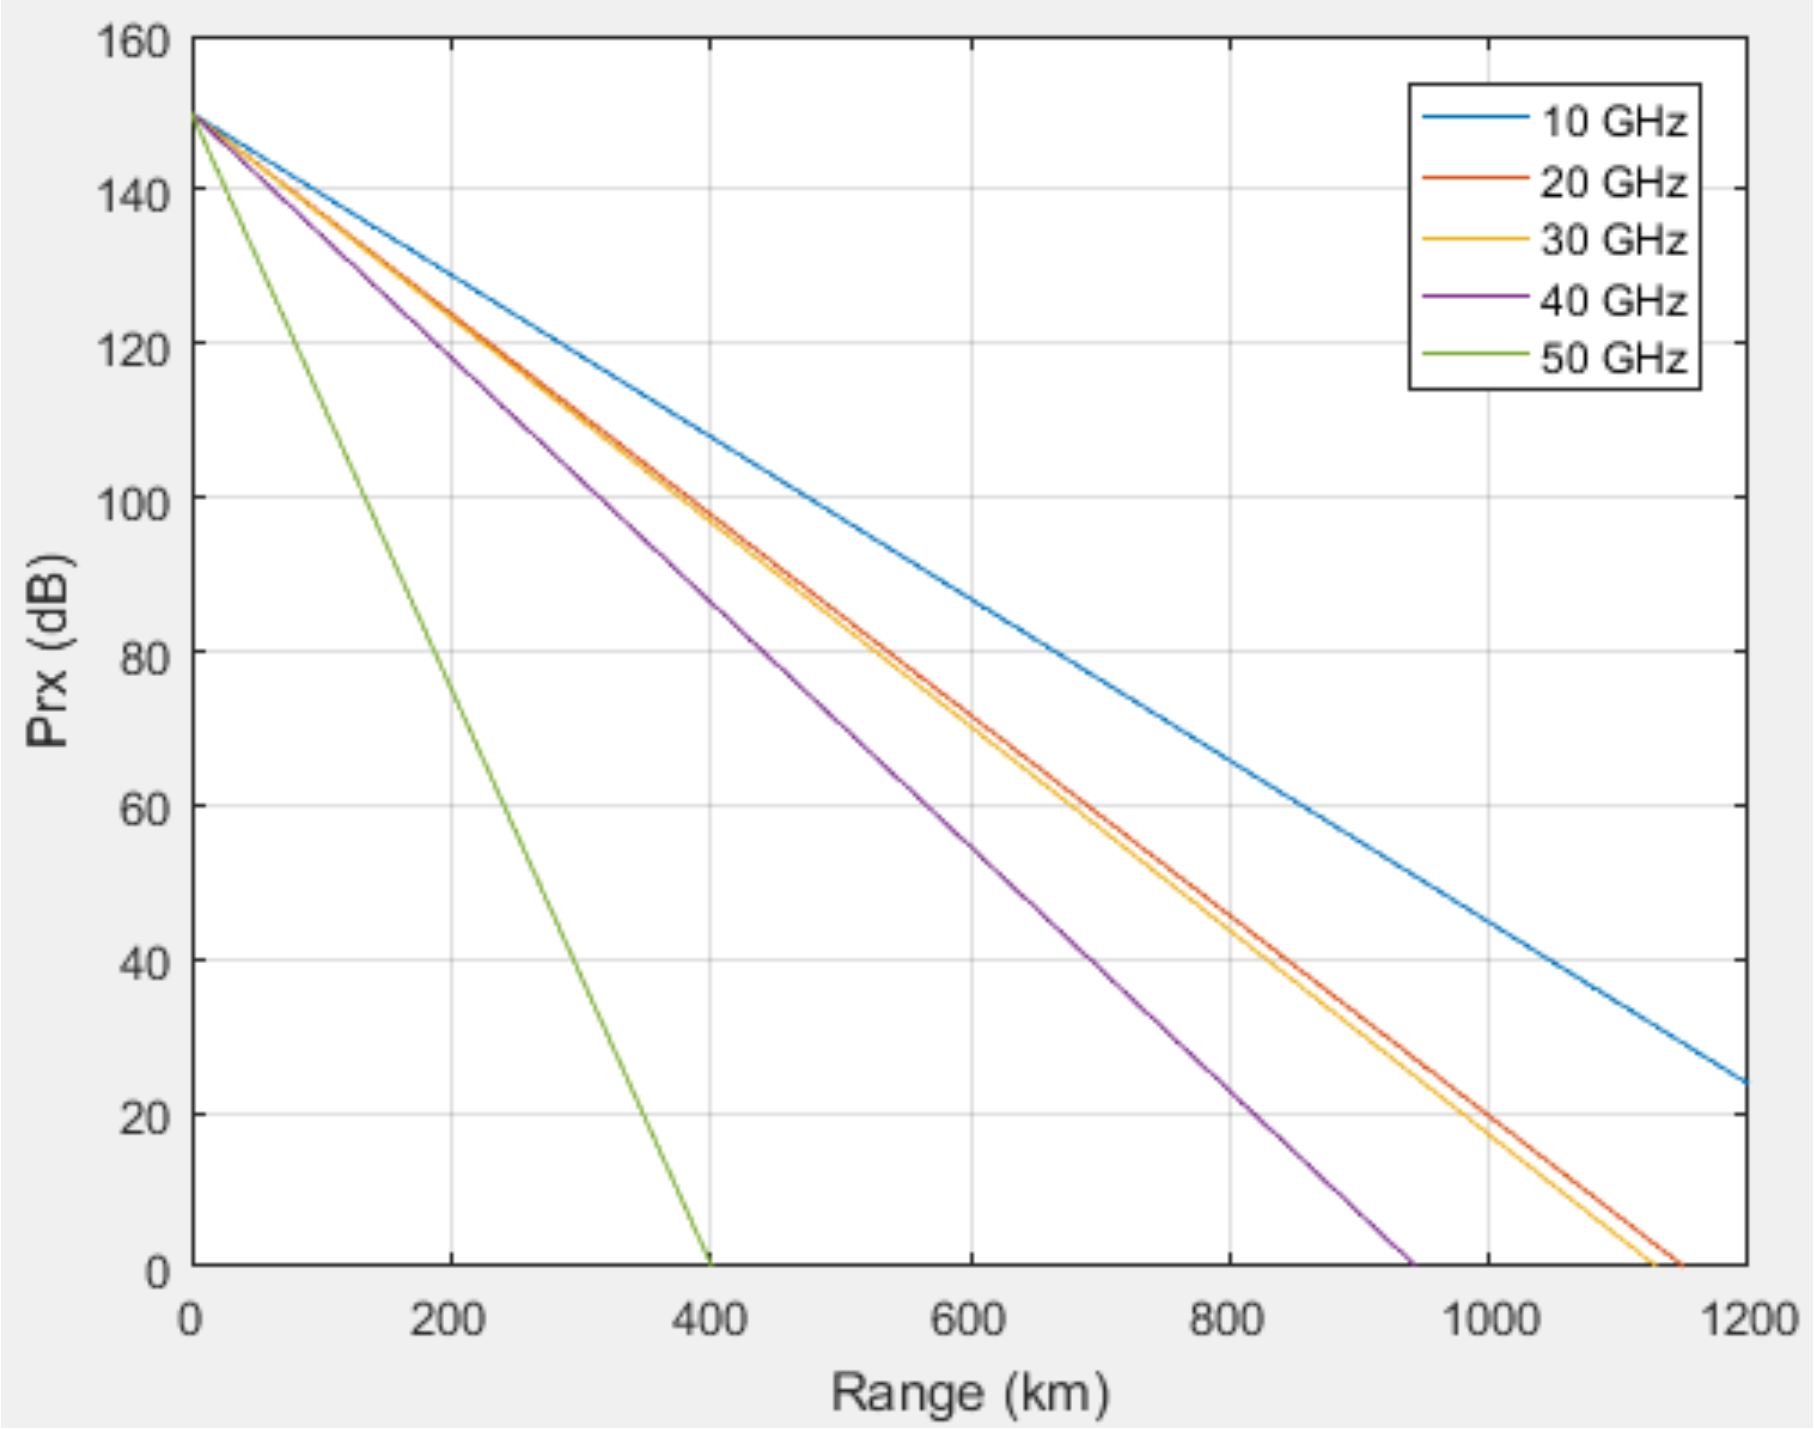
\includegraphics[width=0.8\linewidth]{./res/img/link_budget_w_ecc.png}
  \caption{Link budget con \ac{ECC}}
  \label{fig:link-budget-w-ecc}
\end{figure}

Per assicurare la minima probabilità d'errore è necessario avere un margine del \ac{SNR} al ricevitore, che dipende dal tipo di modulazione.
Dalla figura \ref{fig:link-budget-w-ecc} possiamo vedere che ad alte frequenze l'altezza dell'oribita è limitata a 340 km.
Il lancio della maggior parte dei satelliti è pianificata a quest'altezza.
Per frequenze più basse, possono essere utilizzate orbite più alte a 550 km e 1110 km \cite{rozenvasser_estimation_2023}.

\subsection{Binary Phase Shift Keying (BPSK)}
\ac{BPSK} è la forma più semplice di phase shift keying (\ac{PSK}).
Utilizza due fasi, che sono separate da 180$\degree$ e quindi può essere anche chiamata 2-\ac{PSK}
Non importa particolarmente dove i punti sono posizionati nella costellazione, e in figura \ref{fig:bpsk-diagram} sono posizionati sull'asse dei reali, rispettivamente a 0$\degree$ e 180$\degree$.
La costellazione è la più robusta di tutte le \ac{PSK}, ma può solo modulare 1 bit/simbolo e non è quindi adatta per applicazioni ad alta velocità di trasmissione dati.

\begin{figure}[htbp]
  \centering
  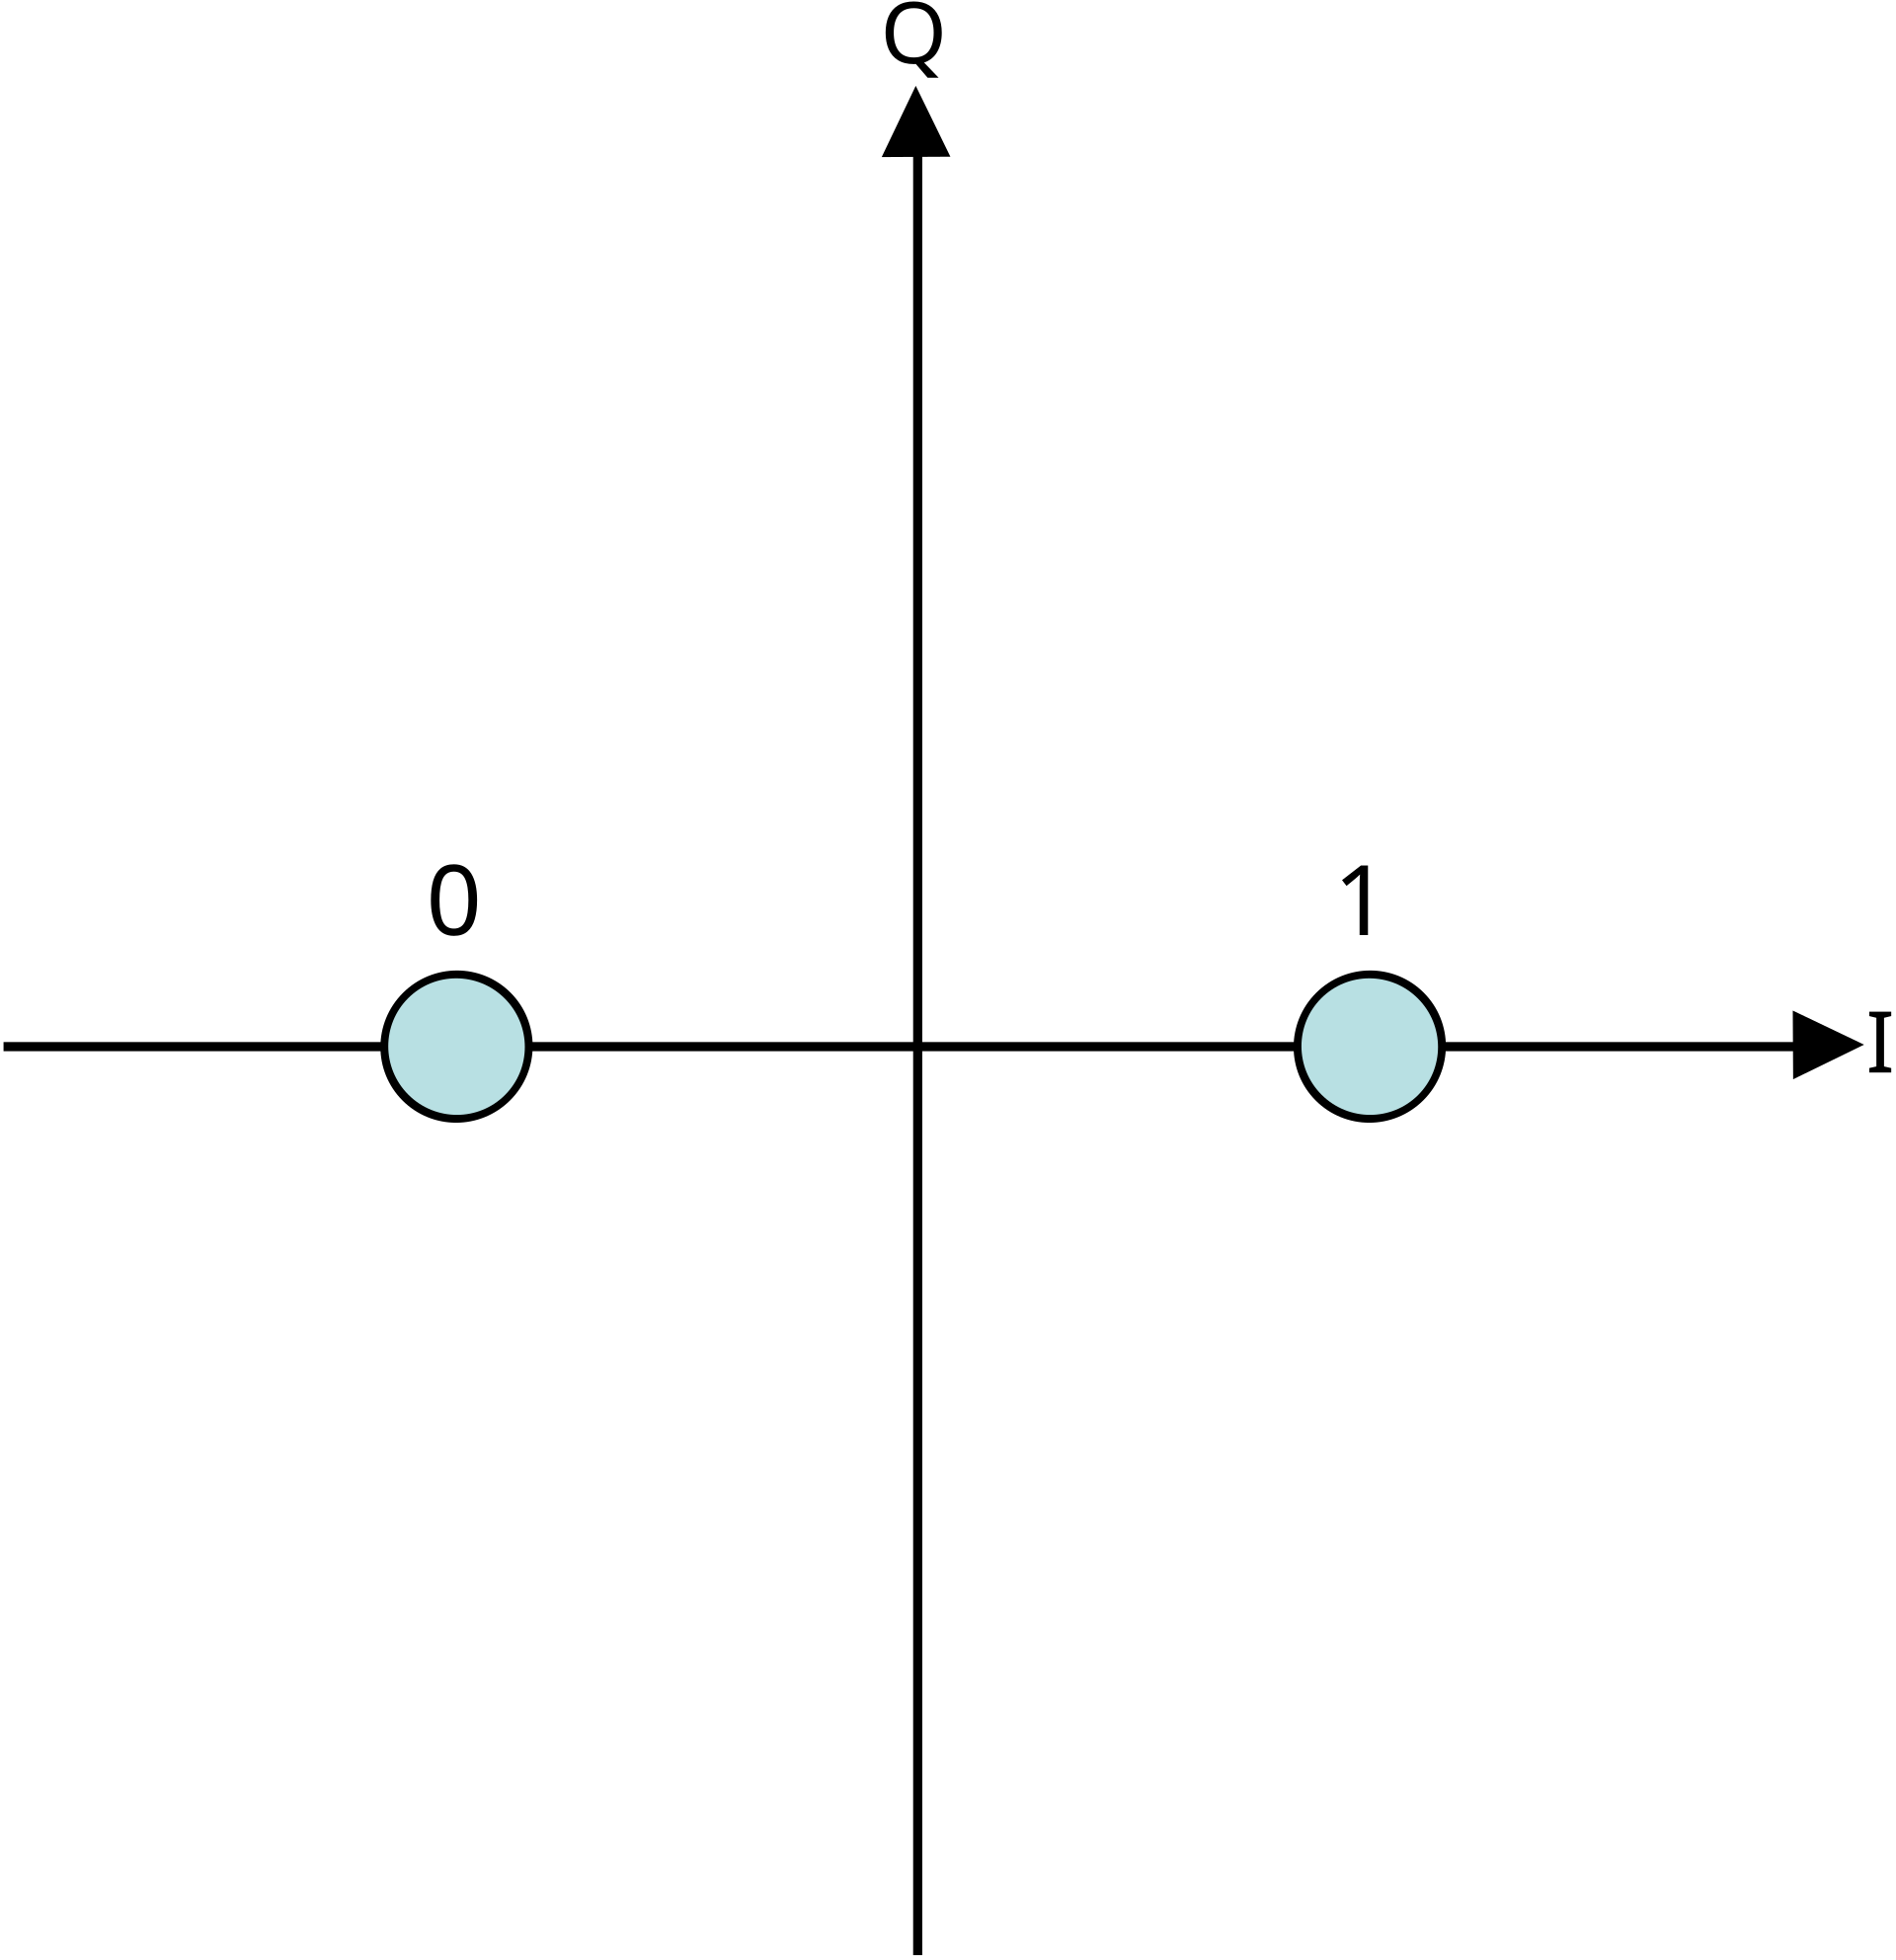
\includegraphics[width=0.4\linewidth]{./res/img/bpsk_diagram.png}
  \caption{Diagramma per la costellazione BPSK}
  \label{fig:bpsk-diagram}
\end{figure}

La forma generale per la \ac{BPSK} segue l'equazione: $$s_n(t) = \sqrt{\frac{2E_b}{T_b}} \cos(2\pi f t + \pi(1-n)) \quad , n = 0,1 $$.
Questo dà due fasi: 0 e $\pi$.

Il bit error rate (\ac{BER}) della \ac{BPSK} sotto ipotesi di rumore addittivo Gaussiano bianco (\ac{AWGN}) può essere calcolata come: $P_b = Q(\sqrt{\frac{2 E_b}{N_0}})$.

Per la \ac{BPSK}, probabilità di errore sul bit è espressa come: $P_{\text{bit}} = \frac{1}{2} erfc(\sqrt{\frac{E_b}{N_0}})$.

\subsection{Quadrature Phase Shift Keying (QPSK)}
A volte viene chiamata anche 4-\ac{PSK}, o 4-\ac{QAM} (anche se i concetti alla base sono diversi le onde radio risultanti sono esattamente le stesse).
La \ac{QPSK} utilizza quattro punti sul diagramma delle costellazioni, equispaziate attorno a un cerchio.
Con quattro fasi, \ac{QPSK} può codificare due bit per simbolo, utilizzando la codifica di Gray per minimizzare il bit error rate (\ac{BER}).

Si può anche utilizzare una \ac{QPSK} per raddoppiare il data rate rispetto a una \ac{BPSK} utilizzando la stessa banda, oppure per mantenere lo stesso data rate di una \ac{BPSK} ma dimezzando la banda richiesta.
Nel secondo caso, il \ac{BER} di una \ac{QPSK} è esattamente lo stesso \ac{BER} di una \ac{BPSK}.

\begin{figure}[htbp]
  \centering
  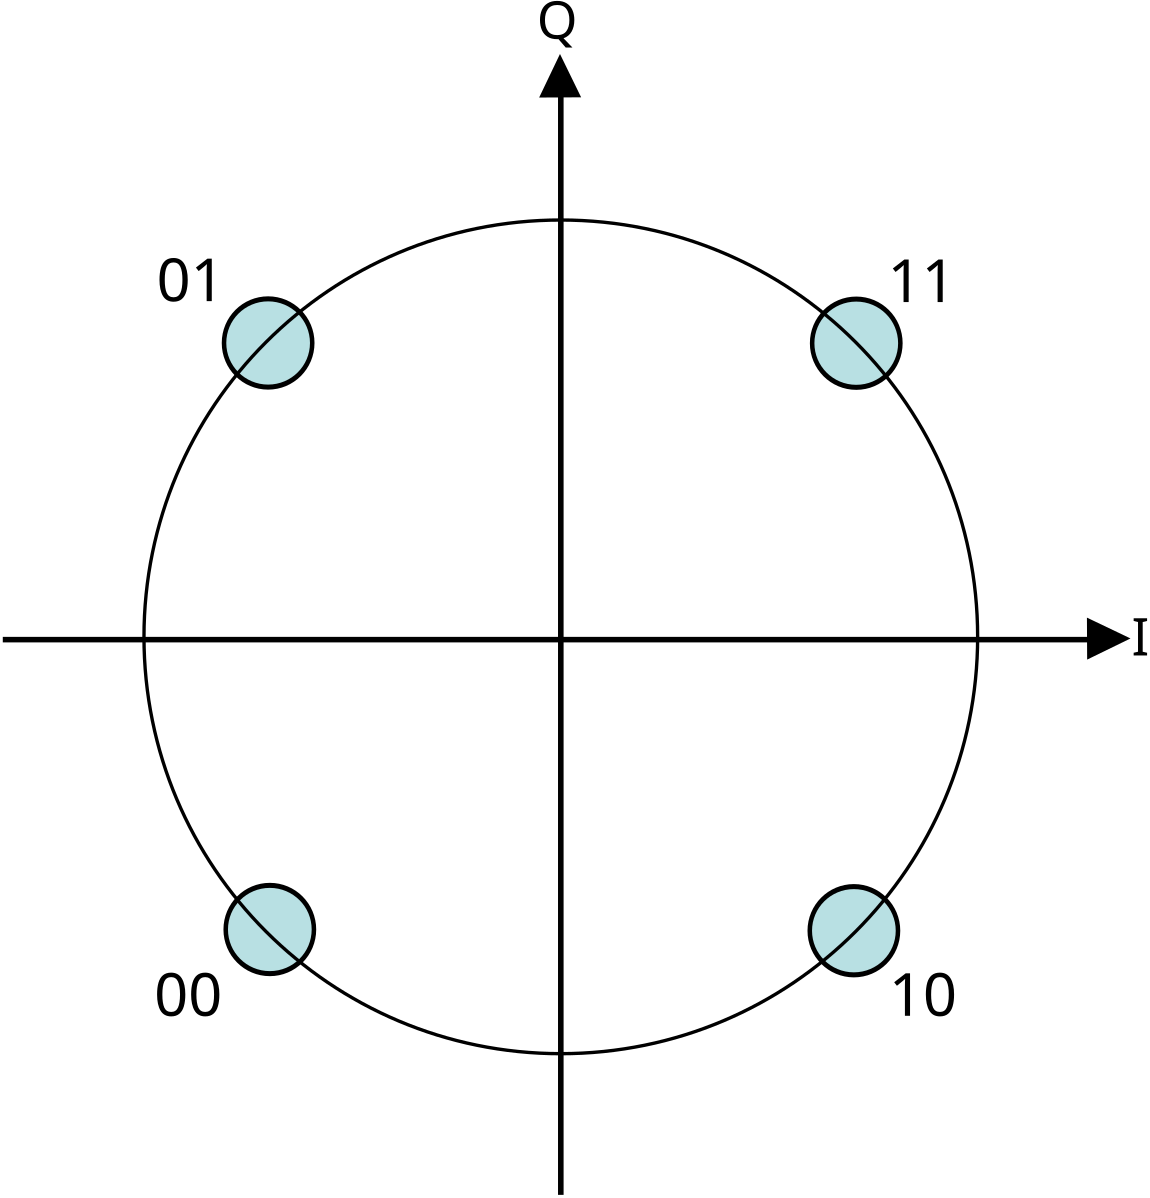
\includegraphics[width=0.4\linewidth]{./res/img/qpsk_diagram.png}
  \caption{Diagramma per la costellazione QPSK}
  \label{fig:qpsk-diagram}
\end{figure}

L'implemetazione di una \ac{QPSK} è più generale di quella di una \ac{BPSK}.
L'equazione dei punti della costellazione è: $$s_n(t) = \sqrt{\frac{2 E_s}{T_s}} \cos(2 \pi f_c t + (2n - 1)\frac{\pi}{4}) \quad , n=1,2,3,4$$.

Da questa formula otteniamo le fasi: $\frac{\pi}{4},\frac{3\pi}{4},\frac{5\pi}{4},\frac{7\pi}{4}$.

Questo risulta in un segnale bidimensionale con base ortonormale: $$\phi_1(t) = \sqrt{\frac{2}{T_s}} \cos(2 \pi f_c t) \quad, \phi_2(t) = \sqrt{\frac{2}{T_s}} \sin(2 \pi f_c t)$$.
La prima componente della base viene utilizzata come fase del segnale, e la seconda componente come quadratura.
Quindi, i segnali della costellazione corrispondono ai 4 punti $(\pm \sqrt{\frac{E_s}{2}}, \pm \sqrt{\frac{E_s}{2}})$.
I fattori di $\frac{1}{2}$ indicano che la potenza totale è distribuita equamente tra le due portanti.

Comparare i segnali della base con quelli della \ac{BPSK} mostra chiaramente come la \ac{QPSK} può essere vista come due segnali \ac{BPSK} indipendenti.

Anche se la \ac{QPSK} può essere vista come una modulazione quaternaria, è più semplice vederla come due portanti in quadratura modulate indipendentemente.
Con questa interpretazione, i bit pari (o dispari) vengono utilizzati per modulare la componente in fase della portante, mentre i bit dispari (o pari) vengono utilizzati per modulare la compornente in quadratura-fase della portante.
\ac{BPSK} viene utilizzato su entrambe le portanti e possono essere demodulate indipendentemente.

Come risultato, la probabilità di errore della \ac{QPSK} è la stessa della \ac{BPSK}, cioè: $P_b = Q(\sqrt{\frac{2 E_b}{N_0}})$

La differenza è che, per raggiungere la stessa probabilità di errore sul bit della \ac{BPSK}, la \ac{QPSK} utilizza il doppio della potenza (dato che due bit sono trasmessi simultaneamente).

La probabilità di errore sul simbolo è data da:
$$P_s = 1 - (1-P_b)^2 = 2Q(\sqrt{\frac{E_s}{N_0}}) - [Q(\sqrt{\frac{E_s}{N_0}})]^2$$

Se il rapporto segnale rumore è alto la probabilità di errore sul simbolo può essere approssimata come:
$$P_s \approx 2Q(\sqrt{\frac{E_s}{N_0}})$$

\subsubsection{Offset Quadrature Phase Shift Keying (OQPSK)}
Starlink utilizza però la \ac{OQPSK}, che è una variante della modulazione phase-shift keying che utilizza quattro diversi valori di fase da trasmettere.
Prendere quattro valori di fase alla volta per costruire un simbolo \ac{QPSK} può consentire alla fase del segnale di saltare fino a $180 \degree$ alla volta.
Quando il segnale è filtrato passa-basso, questi sfasamenti determinano grandi fluttuazioni di ampiezza, una proprietà non desiderabile nei sistemi di comunicazione.
Se compensiamo la temporizzazione dei bit pari e dispari di un periodo di un bit, o mezzo periodo di simbolo, le componenti in fase e in quadratura non cambieranno mai contemporaneamente.
Nel diagramma della costellazione in figura \ref{fig:oqpsk-diagram}, si può vedere che questo limiterà lo sfasamento a non più di $90 \degree$ alla volta.
Ciò produce fluttuazioni di ampiezza molto inferiori rispetto al \ac{QPSK} non offset e talvolta è preferito nella pratica.

\begin{figure}[htbp]
  \centering
  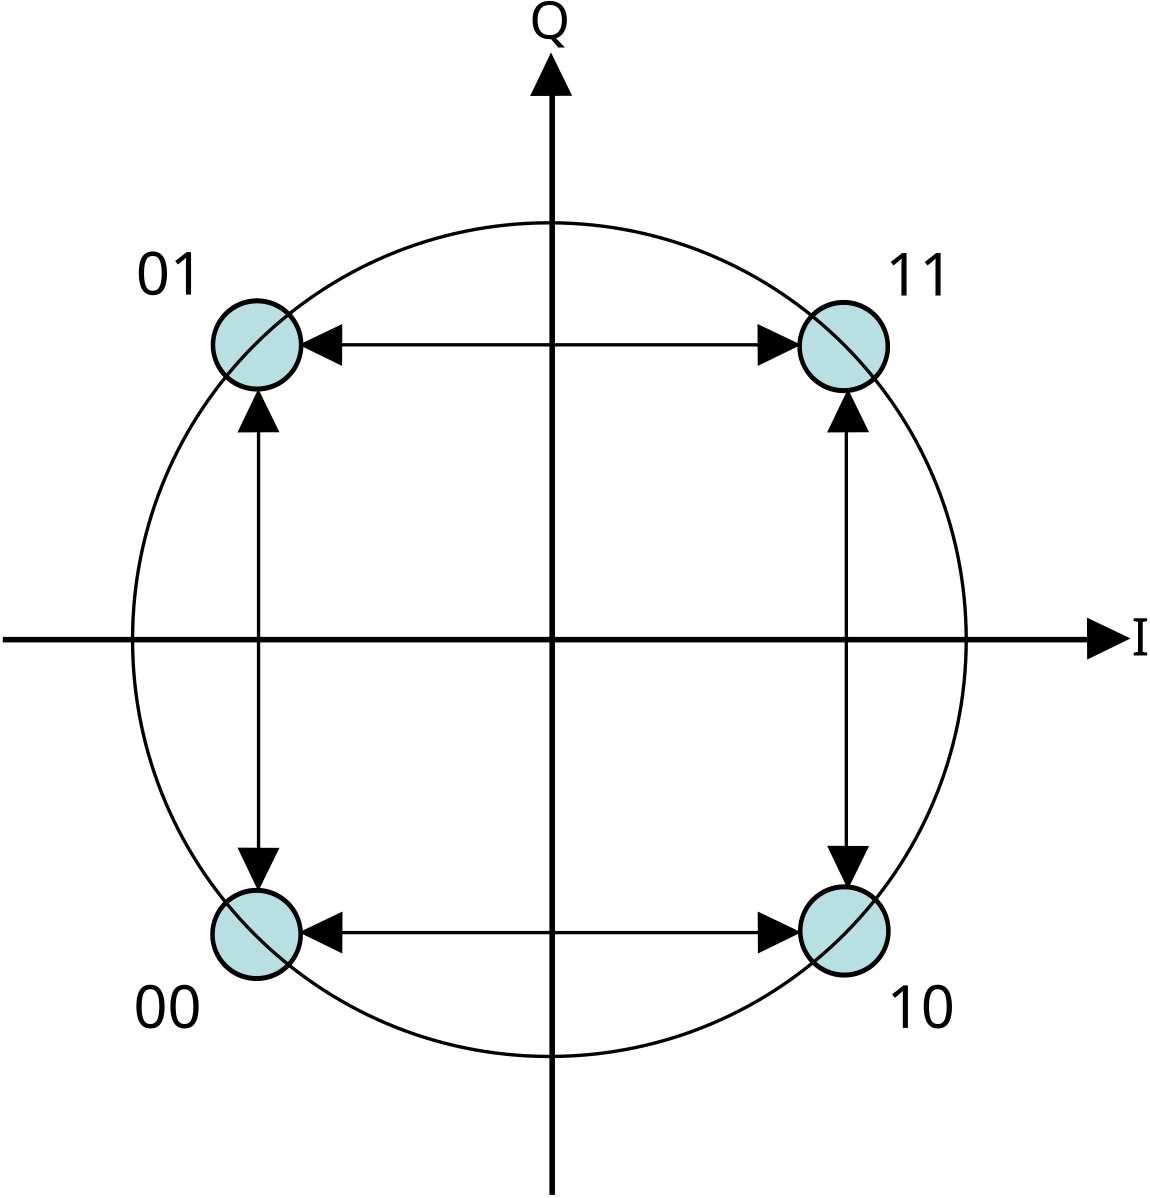
\includegraphics[width=0.4\linewidth]{./res/img/oqpsk_diagram.png}
  \caption{Diagramma per la costellazione OQPSK}
  \label{fig:oqpsk-diagram}
\end{figure}

\subsection{Quadrature Amplitude Modulation (QAM)}
La modulazione \ac{QAM} trasmette segnali modulando le ampiezze di due onde portanti, utilizzando lo schema di modulazione digitale amplitude-shift keying (ASK) o lo schema di modulazione analogica amplitude modulation (AM). Le due onde portanti hanno la stessa frequenza e sono fuori fase tra loro di $90\degree$.
Il segnale trasmesso è creato sommando le due onde portanti tra di loro.
Al ricevitore, le due onde possono essere coerentemente demodulate grazie alla loro ortogonalità.
Nella \ac{QAM}, i punti della costellazione sono distribuiti in una griglia quadrata con spaziatura orizzontale e verticale uguale.

Utilizzando una costellazione di ordine superiore è possibile trasmettere più bit per simbolo.
Però, se l'energia media della costellazione è la stessa, i punti devono essere più vicini tra di loro e quindi più suscettibili al rumore.
Questo risulta in un \ac{BER} più alto, e quindi costellazioni di ordine superiore possono fornire dati in modo meno affidabile rispetto alle costellazioni di ordine inferiore, con un'energia media costante.
Utilizzare \ac{QAM} di ordine più alto senza aumentare il \ac{BER} richiede un più alto \ac{SNR}, che si ottiene aumentando l'energia del segnale, riducendo il rumore, o facendo entrambe le cose.

Se sono richieste velocità di trasmissione dati superiori a quelle offerte da 8-\ac{PSK}, è più conveniente passare a \ac{QAM} poichè consente di ottenere una distanza maggiore tra i punti adiacenti nel piano complesso distribuendo i punti in modo più uniforme.
Il fattore che complica le cose è che i punti non sono più tutti alla stessa ampiezza e quindi il demodulatore deve identificare correttamente sia la fase che l'ampiezza, e non solo la fase.

\section{Direzionamento del traffico}
Starlink direziona il traffico dai terminali utenti alle ground station in un processo a due step.

\begin{figure}[htbp]
  \centering
  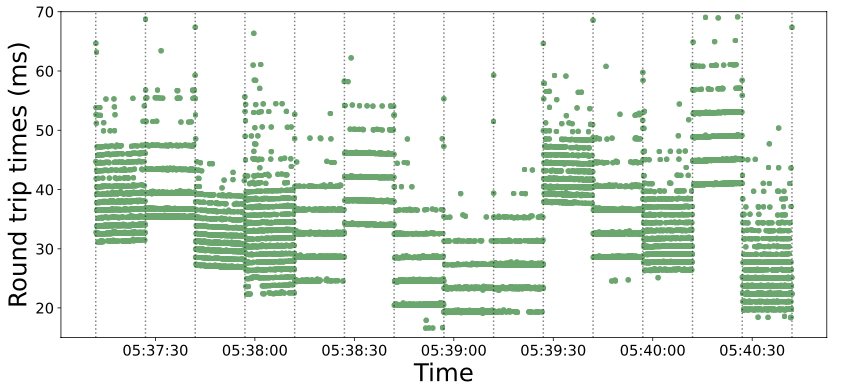
\includegraphics[width=0.8\linewidth]{./res/img/rtt_euterminal.png}
  \caption{\ac{RTT} misurato da un terminale in Europa \cite{tanveer_making_2023}}
  \label{fig:rtt-euterminal}
\end{figure}

Come prima cosa un controller globale di rete, che alloca i satelliti ai terminali degli utenti basandosi su fattori quali il carico (inteso come banda del satellite occupata da altri utenti), le condizioni geospaziali (principalmente visibilità del satellite dal terminale utente e condizioni atmosferiche), e carica del satellite.
Da come si può vedere in figura \ref{fig:rtt-euterminal} i cambiamenti di latenza misurati avvengono ogni 15 secondi, e quindi le allocazioni vengono fatte ogni 15 secondi.

Come seconda cosa c'è un controller nel satellite, che pianifica i flussi dai terminali utente assegnati a un satellite specifico.
Questo si può notare dalla presenza di bande di latenza parallele negli intervalli di 15 secondi di allocazione dei terminali al satellite \cite{tanveer_making_2023} \cite{geoff_huston_transport_2024}.

Misure successive hanno rivelato che il servizio ha una velocità di download mediana di circa 120 Mbps in download, con picchi di 370 Mbps e minimi di 10 Mbps, e 15 Mbps di capacità in upload, con varianza tra i 5 Mbps e i 50 Mbps, come si può vedere in figura \ref{fig:starlink-performance} \cite{geoff_huston_transport_2024}.

\begin{figure}[htbp]
  \centering
  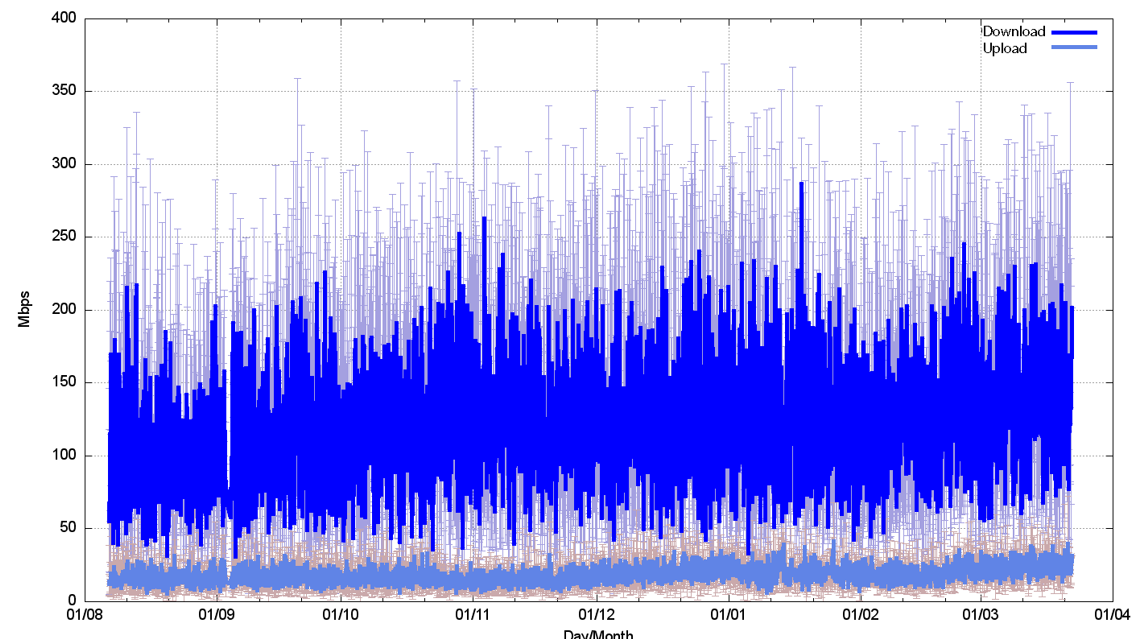
\includegraphics[width=0.7\linewidth]{./res/img/starlink_performance.png}
  \caption{Performance misurate da agosto 2023 a marzo 2024}
  \label{fig:starlink-performance}
\end{figure}

Varianti tradizionali del \ac{TCP}, come Reno, faticano nell'ambiente delle comunicazioni satellitari, dato che utilizzano un'inflazione lineare della finestra di invio mentre non ci sono perdite, e dimezza la sua dimensione come risposta al packet loss.
Varianti moderne come CUBIC hanno performance migliori grazie al Selective Acknowledgement (SACK), che gli permette di differenziare packet loss isolati da una congestione di rete, e utilizza un "window inflation rate" variabile che tenta di stabilizzare il tasso di invio a un livello subito sotto la costruzione delle code di rete (che porta poi al packet loss).

In termini generali c'è un piccolo insieme di ipotesi comuni sulle caratteristiche del percorso di rete per questi algoritmi di controllo TCP.
\begin{itemize}
  \item Esiste una capacità massima stabile del percorso, dove il termine stabilità descrive una situazione in cui la capacità del percorso disponibile è relativamente costante su diversi intervalli di tempo di andata e ritorno (RTT).
  \item La quantità di jitter (variazione nel ritardo end-to-end) è bassa in proporzione all'RTT.
  \item Il tasso medio di perdita di pacchetti è basso. Nel caso di algoritmi di controllo TCP basati sulla perdita di pacchetti, la perdita di pacchetti è generalmente interpretata dall'algoritmo come un segno che i buffer della rete si sono riempiti e la perdita è un'indicazione di buffer overflow.
\end{itemize}

Ovviamente, come abbiamo notato, le prime due condizioni non valgono necessariamente per i percorsi end-to-end che includono un componente Starlink.
Anche il profilo di perdita è diverso.
Esiste la possibilità di una perdita di pacchetti indotta dalla congestione, come nel caso di qualsiasi mezzo a commutazione di pacchetto non sincrono, ma c'è una componente di perdita aggiuntiva che può verificarsi durante il trasferimento satellitare e un'ulteriore componente di perdita che può essere causata da altri problemi causati al segnale radio.

Il TCP in genere tende a reagire a tali ambienti utilizzando scelte conservative.

Anche il verificarsi di una perdita di pacchetti non basata sulla congestione può compromettere le prestazioni TCP. Convenzionalmente, la perdita indurrà il mittente a ridurre rapidamente la sua finestra di invio, sulla base del fatto che se questa perdita è causata da un overflow del buffer di rete, il mittente deve consentire a questi buffer di svuotarsi e quindi riprenderà a inviare a una velocità inferiore, il che dovrebbe ripristinare la coerenza del ciclo di controllo del feedback.

BBR, un algoritmo di controllo di congestione sviluppato da Google, ha dimostrato performance promettenti su Starlink mantenendo il tasso di invio anche durante la perdita di pacchetti.
L'algoritmo stima il prodotto banda-ritardo del percorso e aggiusta i tassi di invio basandosi sui cambiamenti di latenza.
Il problema di questo algoritmo è che la sua richiesta aggressiva di risorse può affamare le altre sessioni TCP \cite{geoff_huston_transport_2024}.

\subsection{Identificazioni delle allocazioni del satellite}
Per studiare l'algoritmo di scheduling, i ricercatori hanno dovuto identificare a quale satellite si connettevano i terminali utente.
Usando le mappe di ostruzione fornite dall'applicazione per smartphone di Starlink hanno usato una nuova tecnica per trovare la traiettoria dei satelliti a cui un terminale si è connesso di recente.
Il processo è sviluppato come segue:
\begin{enumerate}
  \item Estrarre le mappe di ostruzione 2D ogni 15 secondi usando \verb|starlink-grpc-tools| (che è una libreria per eseguire comandi su altri computer come se fossero eseguiti in locale) e ottenendo le posizioni dei satelliti disponibili pubblicamente.
  \item Allineare le mappe 2D con le mappe 3D nell'app di starlink per determinare i parametri delle mappe 2D, come centro, raggio, e la rappresentazione degli angoli di elevazione e azimuth.
  \item Isolare la traiettoria del satellite connesso durante uno slot di 15 secondi specifico facendo delle considerazioni sulle mappe di ostruzione dallo slot precedente e quello attuale.
  \item Identificare il satellite che serve il terminale utente comparando le traiettorie estratte con la posizione calcolata dei satelliti visibili usando la misura di distanza Dynamic Time Warping, che è un modo di confrontare due sequenze temporale che non sono perfettamente sincronizzate.
\end{enumerate}

\subsection{Caratteristiche e preferenze dello scheduler globale}
Le analisi dei satelliti allocati hanno rivelato diverse preferenze dello scheduler globale. Si possono individuare tre fattori determinanti per la scelta:
\begin{itemize}
  \item Posizione del satellite: lo scheduler preferisce satelliti con angoli di elevazione più alti, con la mediana dei satelliti selezionati a 22.9 gradi più alta di quelli non selezionati \cite{tanveer_making_2023}.
  Lo scheduler ha anche una preferenza per i satelliti a nord del terminale utente. Questo probabilmente è dovuto alla zona di esclusione dell'International Telecommunication Union per le orbite geostazionarie e considerazioni di efficienza energetica, dato che i satelliti con un angolo di elevazione più alto hanno bisogno di meno energia per la comunicazione \cite{tanveer_making_2023}.
  \item Data di lancio del satellite: lo scheduler dà priorità ai satelliti più nuovi, infatti la probabilità che un satellite sia selezionato aumenta all'aumentare della sua data di lancio. Questa preferenza potrebbe essere legata al mantenimento di una copertura stabile della costellazione, dato che i satelliti più vecchi stanno raggiungendo la fine del loro ciclo di vita.
  \item Stato di illuminazione: lo scheduler favorisce i satelliti illuminati dal sole, scegliendoli il 72.3\% delle volte quando sono disponibili sia satelliti illuminati che non. I satelliti non illuminati sono selezionati solo quando rappresentano almeno il 35\% dei satelliti disponibili. La scelta sembra comunque guidata dal fatto che il loro angolo di elevazione sia maggiore di quelli illuminati, probabilmente per risparmiare energia \cite{tanveer_making_2023}.
\end{itemize}

\section{Comparazione della struttura del segnale con sistemi terrestri OFDM}
La struttura del segnale inviato da Starlink utilizza \ac{OFDM}, una scelta popolare pre i sistemi di comunicazione wireless, come Wi-Fi e LTE.
Tuttavia, il progetto di starlink differisce dai sistemi usati sulla terra per diversi aspetti chiave, che riflettono le caratteristiche uniche del canale di comunicazione spazio-terra e gli obiettivi di Starlink.

\paragraph{Layout di canale} A differenza dei sistemi terresti dove la larghezza di banda e gli schemi di duplexing variano a livello regionale, Starlink impiega una struttura coerente per il downlink in banda Ku, con otto canali da 240 MHz separati da bande di guardia da 10 MHz.
Questa ampia banda di guardia consente di attivare più canali contemporaneamente all'interno di una cella di servizio e riduce al minimo le interferenze tra celle adiacenti.
In questo modo si riduce potenzialmente l'efficienza spettrale, ma si migliora l'affidabilità \cite{humphreys_signal_2023}.

\paragraph{Layout dei frame}
I frame inviati da starlink, con un periodo di 1/750 secondi, seguono un layout consistenza con un'alta proporzione di sequenze di sincronizzazione; la PSS, SSS, CM1SS e CSS.
Questa enfasi sulla sincronizzazione, superiore a quella dell'LTE e di altri sistemi terrestri, consente un'accurata equalizzazione del canale e stima dell'effetto Doppler, migliorando potenzialmente l'affidabilita della comunicazione e consentendo un doppio uso per il PNT (Positioning Navigation e Timing) \cite{humphreys_signal_2023}.

\paragraph{Sequenze di sincronizzazione}
L'utilizzo di sequenze di sincronizzazione multiple per frame, includendo il PSS m-sequence-based e la 4-\ac{QAM}-modulated SSS, lo distingue dai tradizionali sistemi terresti.
L'utilizzo di queste sequenze di sincronizzazione e la scelta di un numero moderato di sottoportatori semplificano l'elaborazione del segnale e garantiscono una sincronizzazione robusta anche in condizioni difficili \cite{humphreys_signal_2023}.

\paragraph{Efficienza e margini di design}
La struttura del segnale Starlink prioritizza l'affidabilità.
L'efficiente occupazione dei simboli OFDM sfrutta il basso ritardo del canale \ac{LEO}-terra.
Le ampie bande di guardia e l'elevata occupazione dei frame, pur riducendo l'efficienza spettrale, migliorano la mitigazione delle interferenze e la precisione della sincronizzazione.
La scelta di un numero relativamente basso di sottoportanti (N = 1024) indica un design che prioritizza la robustezza piuttosto che massimizzare il throughput teorico \cite{humphreys_signal_2023}.

